\pdfoutput=1
\documentclass[a4paper,pdflatex,ja=standard]{bxjsarticle}

% ---Setting about the geometry of the document----
% \usepackage{a4wide}
% \pagestyle{empty}

% ---Physics and Math Packages---
\usepackage{amssymb,amsfonts,amsthm,mathtools}
\usepackage{physics,braket,bm}

% ---underline---
\usepackage{ulem}

% --- sorround the texts or equations
% \usepackage{fancybox,ascmac}

% ---settings of theorem environment---
% \usepackage{amsthm}
% \theoremstyle{definition}

% ---settings of proof environment---
% \renewcommand{\proofname}{\textbf{証明}}
% \renewcommand{\qedsymbol}{$\blacksquare$}

% ---Ignore the Warnings---
\usepackage{silence}
\WarningFilter{latexfont}{Some font shapes,Font shape}

% ---Insert the figure (If insert the `draft' at the option, the process becomes faster)---
% \usepackage{graphicx}
% \usepackage{subcaption}

% ----Add a link to a text---
\usepackage{url}
\usepackage{xcolor,hyperref}
\hypersetup{colorlinks=true,citecolor=orange,linkcolor=blue,urlcolor=magenta}
\usepackage{bxcjkjatype}

% ---Tikz---
\usepackage{tikz,pgf,pgfplots,circuitikz}
\pgfplotsset{compat=1.15}
\usetikzlibrary{intersections,arrows.meta,angles,calc,3d,decorations.pathmorphing}

% ---Add the section number to the equation, figure, and table number---
\makeatletter
   \renewcommand{\theequation}{\thesection.\arabic{equation}}
   \@addtoreset{equation}{section}
   
   \renewcommand{\thefigure}{\thesection.\arabic{figure}}
   \@addtoreset{figure}{section}
   
   \renewcommand{\thetable}{\thesection.\arabic{table}}
   \@addtoreset{table}{section}
\makeatother

% ---enumerate---
\renewcommand{\labelenumi}{$(\arabic{enumi})$}
% \renewcommand{\labelenumii}{$(\arabic{enumii})$}

% ---Index---
% \usepackage{makeidx}
% \makeindex 

% ---Fonts---
\renewcommand{\familydefault}{\sfdefault}

% ---Title---
\title{早稲田大学\ 2022年\ 物理学専攻\ 院試\ 解答例}
\author{ミヤネ}
\date{最終更新:\today}

\newcommand{\prb}[2]{
  \clearpage
  \phantomsection
  \addcontentsline{toc}{section}{問題 #1: #2}
  \section*{問題番号\fbox{#1}\ (#2)}
  \setcounter{section}{#1}
  \setcounter{equation}{0}
}

\begin{document}

\maketitle

\tableofcontents
\clearpage

\prb{1}{微積分}

\begin{enumerate}
  \item 
  $\alpha>0$のときに絶対収束する.

  \begin{proof}
    \uline{$0<\alpha<1$のとき}

    このときは$t=0$が特異点なので,
    \begin{equation}
      \int_{0}^{1}
      e^{-t}t^{\alpha-1}
      \dd t
      \label{int_0to1}
    \end{equation}
    の収束性を評価してやればよい.$0<t<1$では,次の不等式
    \begin{equation}
      e^{-t}t^{\alpha-1}<t^{\alpha-1}
    \end{equation}
    が成立しており,右辺を$0<t<1$で積分すると
    \begin{equation}
      \int_{0}^{1}
      t^{\alpha-1}
      \dd t
      =
      \frac{1}{\alpha}
      <
      \infty
    \end{equation}
    なので,積分\eqref{int_0to1}は収束する.
    \\

    \uline{$\alpha>1$のとき}

    このときは$t\rightarrow\infty$が特異点なので,
    \begin{equation}
      \int_{s}^{\infty}
      e^{-t}t^{\alpha-1}
      \dd t
      \label{int_1toinfinity}
    \end{equation}
    を評価すればよい.なお,$s$は
    \begin{equation}
      e^{-2s}s^{\alpha-1}
      =
      1
    \end{equation}
    となるような正の実数であり,このような$s$は,中間値の定理より保証される.関数$e^{-t}t^{\alpha-1}$は単調減少なので$t>s$では
    \begin{gather}
      e^{-2t}t^{\alpha-1}<1
      \\
      \therefore
      e^{-t}t^{\alpha-1}
      <
      e^{-t}
    \end{gather}
    である.したがって,積分(\ref{int_1toinfinity})は
    \begin{equation}
      \int_{s}^{\infty}
      e^{-t}t^{\alpha-1}
      \dd t
      <
      \int_{s}^{\infty}
      e^{-t}
      \dd t
      =
      \frac{1}{e^{s}}
      <
      \infty
    \end{equation}
    となり,収束する.
  \end{proof}

  \item 
  $0<\theta<1$のときに収束する\footnote{
    さぼります.
  }.

  \item 
  被積分関数を
  \begin{equation}
    f(z)
    \coloneqq
    \frac{z^{-\theta}}{1+z}
    \label{integral}
  \end{equation}
  としておく.この$f(z)$を図\ref{contour}で積分する.積分で重要な部分は$\Gamma_{1},\Gamma_{2}$なので,その部分を評価する\footnote{
    他の部分は収束します.
  }.すると,
  \begin{equation}
    \int_{\Gamma_{1}}f
    +
    \int_{\Gamma_{2}}
    =
    2\pi i\Res[f,-1]
  \end{equation}
  となるので,それぞれの項を評価してやればよい.まず,$\Gamma_{1}$での積分は,普通に
  \begin{equation}
    \int_{\Gamma_{1}}f
    =
    \int_{0}^{\infty}
    \frac{x^{-\theta}}{1+x}
    \dd x
    =
    I(\theta)
  \end{equation}
  である.$\Gamma_{2}$の部分は,偏角に注意して
  \begin{equation}
    \int_{\Gamma_{2}}
    =
    \int_{\infty}^{0}
    \frac{x^{-\infty}e^{-2\pi\theta i}}{1+x}
    \dd x
    =
    -
    e^{-2\pi \theta i}I(\theta)
  \end{equation}
  となる.あとは留数を計算して
  \begin{equation}
    2\pi i\Res[f,-1]
    =
    2\pi i e^{-i\pi\theta}    
  \end{equation}
  となるので,
  \begin{equation}
    I(\theta)
    =
    \frac{2\pi i e^{\pi i\theta}}{1-e^{-2\pi i\theta}}
    =
    \frac{\pi}{\sin \theta\pi}
  \end{equation}
  である.

  \begin{figure}[ht]
    \centering    
    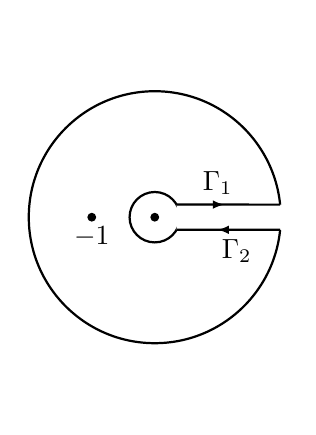
\begin{tikzpicture}[scale=0.8] 
        \draw[thick, name path=C1] (0,0) circle (2);       
        \draw[thick, name path=C2] (0,0) circle (0.4);
        \fill[black] (0,0) circle (2pt);
        \draw [opacity=0.0, name path=line1] (0,0.2)--(2.1,0.2);       
        \draw [opacity=0.0] (0,-3)--(0,3);        
        \draw [opacity=0.0, name path=line2] (0,-0.2)--(2.1,-0.2);
        \draw [name intersections={of= C1 and line1, by={a}}];
        \draw [name intersections={of= C2 and line1, by={b}}];        
        \draw [name intersections={of= C1 and line2, by={c}}];
        \draw [name intersections={of= C2 and line2, by={d}}];
        \fill [white] (d)--(2.1,-0.2)--(2.1,0.2)--(b)--cycle;
        \draw[thick] (d)--(c);
        \draw[thick] (b)--(a);
        \draw (1.0,0.2) node[above]{$\Gamma_{1}$};        
        \draw (1.3,-0.2) node[below]{$\Gamma_{2}$};
        \fill (-1,0) circle (2pt) node[below] {$-1$};
        \draw [-latex, thin] (b)--(1.1,0.2);
        \draw [-latex, thin] (c)--(1.0,-0.2);
      \end{tikzpicture} 
    \caption{(\ref{integral})の積分路}
    \label{contour}
  \end{figure}

  \item 
  $\alpha=1-\theta$とすると
  \begin{equation}
    \Gamma(1-\theta)
    =
    \int_{0}^{\infty}
    e^{-k}k^{-\theta}
    \dd k
  \end{equation}
  である.変数変換$k=st$をすれば
  \begin{equation}
    \Gamma(1-\theta)
    =
    t^{1-\theta}
    \int_{0}^{\infty}
    e^{-st}s^{-\theta}
    \dd s
  \end{equation}
  となる.

  \item 
  前問の結果が任意の$t$>0について用いることができることに注意して,$\Gamma(\theta)$をよく見ると
  \begin{equation}
    \Gamma(\theta)
    =
    \int_{0}^{\infty}
    \frac{e^{-t}}{t^{1-\theta}}
    \dd t
    =
    \int_{0}^{\infty}
    e^{-t}
    \dd t
    \times
    \dfrac{\int_{0}^{\infty}e^{-st}s^{-\theta}\dd s}{\Gamma(1-\theta)}
  \end{equation}
  となっている.よって,
  \begin{equation}
    \Gamma(\theta)\Gamma(1-\theta)
    =
    \uwave{\int_{0}^{\infty}\dd t}\int_{0}^{\infty}\dd s
    \quad
    \uwave{e^{-(s+1)t}}s^{-\theta}
    =
    \int_{0}^{\infty}
    \dd s
    \quad
    \frac{s^{-\theta}}{1+s}
    =
    \frac{\pi}{\sin\theta\pi}
  \end{equation}
  である.

\end{enumerate}





\clearpage
\prb{2}{線形代数・微分方程式}
\begin{enumerate}
  \item 
  $\bm{n}$を左からかけると,$\bm{n}\times\bm{v}(t)$は$\bm{n}$に垂直なので
  \begin{equation}
    \dv{}{t}{(\bm{n}\cdot\bm{v})}(t)
    =
    0
    \ .
  \end{equation}

  \item 
  前問より,$\bm{n}\cdot\bm{v}=\bm{n}\cdot\bm{v}_{0}$なので
  \begin{equation}
    \bm{n}
    \cdot
    (\bm{v}-\bm{v}_{0})
    =
    0
  \end{equation}
  である.したがって,$\bm{v}-\bm{v}_{0}$は$\bm{n}$に垂直な平面上に存在する.よって,$\bm{n}$に垂直な2つのベクトル$\bm{n}\times\bm{v}_{0},\bm{n}\times(\bm{n}\times\bm{v}_{0})$で$\bm{v}-\bm{v}_{0}$が張れるため
  \begin{align}
    \bm{v}(t)
    &=
    \bm{v}_{0}
    +
    \alpha(t)
    \bm{n}\times\bm{v}_{0}
    +
    \beta(t)
    \bm{n}\times(\bm{n}\times\bm{v}_{0})
    \nonumber
    \\
    &=
    (1-\beta(t))\bm{v}_{0}
    +
    \alpha(t)\bm{n}\times\bm{v}_{0}
    +
    \beta(t)(\bm{n}\cdot\bm{v}_{0})\bm{n}
    \label{v_cand}
  \end{align}
  となる.初期条件は
  \begin{equation}
    \alpha(0)
    =
    \beta(0)
    =
    0
  \end{equation}
  である.\eqref{v_cand}を微分方程式に代入すれば
  \begin{equation}
    \left\{
      \begin{alignedat}{1}
        \dv{\bm{v}}{t}
        &=
        -\dv{\beta}{t}\bm{v}_{0}
        +
        \dv{\alpha}{t}\bm{n}\times\bm{v}_{0}
        +
        \dv{\beta}{t}(\bm{n}\cdot\bm{v}_{0})\bm{n}
        \\
        \omega\bm{n}\times\bm{v}(t)
        &=
        \omega\bm{n}\times
        \left\{  
          (1-\beta(t))\bm{v}_{0}
          +
          \alpha\bm{n}\times\bm{v}_{0}
          +
          \beta(t)(\bm{n}\cdot\bm{v}_{0})\bm{n}
        \right\}
        \\
        &=
        -
        \omega\alpha(t)\bm{v}_{0}
        +
        \omega(1-\beta(t))\bm{n}\times\bm{v}_{0}
        +
        \omega\alpha(t)(\bm{n}\cdot\bm{v}_{0})\bm{n}
      \end{alignedat}
    \right.
  \end{equation}
  である.したがって,$\bm{v}_{0},\bm{n}\times\bm{v}_{0},\bm{n}$が1次独立だとすれば
  \begin{equation}
    \left\{
      \begin{alignedat}{1}
        \dv{\alpha}{t}
        &=
        \omega(1-\beta(t))
        \\
        \dv{\beta}{t}
        &=
        \omega\alpha(t)
      \end{alignedat}
    \right.
    \label{diff_eq}
  \end{equation}
  である.第1式を時間で微分して第2式を代入すれば
  \begin{equation}
    \dv[2]{\alpha}{t}
    =
    -\omega^2
    \alpha
  \end{equation}
  なので,初期条件もあわせて考えれば
  \begin{equation}
    \alpha(t)
    =
    \sin\omega t
    \label{alpha}
  \end{equation}
  と解くことができる\footnote{
    ちゃんと解くとなれば
    $$
    \alpha(t)
    =
    A\sin\omega t
    $$
    と定数$A$を用いて書いたほうが正確ですが,$\dot{\bm{v}}(0)=\omega\bm{n}\times\bm{v}_{0}$という初期条件を吟味すれば$A=1$で良いことが分かります.
  }.これを\eqref{diff_eq}の第2式に代入すれば
  \begin{equation}
    \dv{\beta}{t}
    =
    \omega\sin\omega t
  \end{equation}
  であり,初期条件に気をつければ
  \begin{equation}
    \beta(t)
    =
    1-\cos\omega t
    \label{beta}
  \end{equation}
  である.\eqref{alpha},\eqref{beta}を\eqref{v_cand}に代入すれば
  \begin{equation}
    \bm{v}(t)
    =
    \cos\omega t\bm{v}_{0}
    +
    \sin\omega t\bm{n}\times\bm{v}_{0}
    +
    (1-\cos\omega t)(\bm{n}\cdot\bm{v}_{0})\bm{n}
    \label{v_sol}
  \end{equation}  
  となる.

  \item 
  $\bm{v}(t)$を左からかけると,$\bm{n}\times\bm{v}(t)$は$\bm{v}(t)$に垂直なので
  \begin{equation}
    \dv{}{t}{v^2(t)}
    =
    0
  \end{equation}
  となるので
  \begin{equation}
    |\bm{v}(t)|
    =
    |\bm{v}_{0}|
  \end{equation}
  である\footnote{
    \eqref{v_sol}の絶対値を計算してみると
    \begin{align}
      |\bm{v}(t)|^2
      &=
      |\bm{v}_{0}|^2\cos^2\omega t
      +
      \sin^2\omega t(\bm{n}\times\bm{v}_{0})^2
      +
      (1-\cos\omega t)^2(\bm{n}\cdot\bm{v}_{0})^2
      +
      2\cos\omega t(1-\cos\omega t)(\bm{n}\cdot\bm{v}_{0})
      \nonumber
      \\
      &=
      |\bm{v}_{0}|^2\cos^2\omega t
      +
      |\bm{v}_{0}|^2\sin^2\omega t\sin^2\theta
      +
      |\bm{v}_{0}|^2\sin^2\omega t\cos^2 \theta
      \nonumber
      \\
      &=
      |\bm{v}_{0}|^2
      \nonumber
    \end{align}
    となっておりconsistentです.ただし,$\theta$は$\bm{n}$と$\bm{v}_{0}$がなす角です.
  }.

  \item 
  前問の結果より
  \begin{equation}
    |\bm{v}|^{2}
    =
    \bm{v}_{0}^{T}R^{T}(t)
    R(t)\bm{v}_{0}
    =
    \bm{v}_{0}^{T}
    \bm{v}_{0}
  \end{equation}
  が成立していてほしいので,
  \begin{equation}
    R^{T}(t)
    =
    R^{-1}(t)
  \end{equation}
  であればよい.したがって,$R(t)=e^{\varphi(t)G}$と書けば$G$は反対称である.

  \item
  $\bm{v}(t)=R(t)\bm{v}_{0}$を$t$で微分すると
  \begin{equation}
    \dv{\bm{v}}{t}
    =
    \varphi'(t)
    G
    e^{\varphi(t)G}\bm{v}_0
    \label{eq1}
  \end{equation}
  となる.$t=0$を代入すれば
  \begin{equation}
    \dv{\bm{v}(0)}{t}
    =
    \omega G\bm{v}_0
  \end{equation}
  である.一方で,微分方程式を$t=0$とすれば
  \begin{equation}
    \bm{n}\times\bm{v}_0
    =
    G\bm{v}_0
  \end{equation}
  となるので\footnote{
    ちなみに,$\bm{n}=(n_x,n_y,n_z)$に対して
    $$
      G
      =
      \begin{pmatrix}
        0 & -n_z & n_y \\
        n_z & 0 & -n_x \\
        -n_y & n_x & 0
      \end{pmatrix}
    $$
    です.
  },\eqref{eq1}にこの関係を代入すれば
  \begin{equation}
    \dv{\bm{v}}{t}
    =
    \varphi'(t)
    (\bm{n}\times\bm{v})
  \end{equation}
  となっている.よって,$\varphi'(t)\equiv\omega$である.したがって,$\varphi(0)=0$であることに注意すれば\footnote{
    $t=0$で$R(0)=1$なので.
  },$\varphi(t)=\omega t$なので,行列の指数関数の定義から
  \begin{equation}
    \varphi(t)
    =
    \sum_{n=0}^{\infty}\frac{(\omega t)^n}{n!}G^{n}
    =
    1+\omega t G +\mathcal{O}(G^2)
  \end{equation}
  である.

  \item 
  $G$は$SO(3)$のgeneratorなので
  \begin{equation}
    [G^{(i)},G^{(j)}]
    =
    \varepsilon^{ijk}G^{(k)}
    \label{commu_rel}
  \end{equation}
  が成立する.

\end{enumerate}

\subsection*{補足}

\begin{itemize}
  \item 
  さすがに(6)があっけないので,ちょっと計算します.$[G^{(i)},G^{(j)}]$を$\bm{v}_0$に作用させると
  \begin{align}
    [G^{(i)},G^{(j)}]
    \bm{v}_0
    &=
    G^{(1)}G^{(2)}\bm{v}_0
    -
    G^{(2)}G^{(1)}\bm{v}_0
    \nonumber
    \\
    &=
    \bm{n}^{(i)}\times(\bm{n}^{(j)}\times\bm{v}_0)
    -
    \bm{n}^{(j)}\times(\bm{n}^{(i)}\times\bm{v}_0)
    \nonumber
    \\
    &=
    (\bm{n}^{(i)}\cdot\bm{v}_0)\bm{n}^{(j)}
    -
    (\bm{n}^{(j)}\cdot\bm{v}_0)\bm{n}^{(i)}
    \label{commutator}
  \end{align}
  です.ここで,少し唐突ですが,$\varepsilon^{ijk}G^{(k)}\bm{v}_0$という値を計算してみましょう.ここで
  \begin{equation}
    \bm{n}^{(k)}
    =
    \frac{1}{2}\varepsilon^{klm}\bm{n}^{(l)}\times\bm{n}^{(m)}
  \end{equation}
  という関係に注意すれば
  \begin{align}
    \varepsilon^{ijk}G^{(k)}\bm{v}_0
    &=
    \varepsilon^{ijk}
    (\bm{n}^{(k)}\times\bm{v}_0)
    \nonumber
    \\
    &=
    \frac{1}{2}
    \varepsilon^{ijk}
    \varepsilon^{klm}(\bm{n}^{(l)}\times\bm{n}^{(m)})\times\bm{v}_0
    \nonumber
    \\
    &=
    -\frac{1}{2}
    (\delta^{il}\delta^{jm}-\delta^{im}\delta^{jl})
    \left\{  
      (\bm{v}_0\cdot\bm{n}^{(m)})\bm{n}^{(l)}
      -
      (\bm{v}_0\cdot\bm{n}^{(l)})\bm{n}^{(m)}
    \right\}
    \nonumber
    \\
    &=    
    (\bm{n}^{(i)}\cdot\bm{v}_0)\bm{n}^{(j)}
    -
    (\bm{n}^{(j)}\cdot\bm{v}_0)\bm{n}^{(i)}
  \end{align}
  であり,\eqref{commutator}の結果と一致しています.よって,
  \begin{equation}
    [G^{(i)},G^{(j)}]
    \bm{v}_0
    =
    \varepsilon^{ijk}G^{(k)}\bm{v}_0
  \end{equation}
  なので,\eqref{commu_rel}が成立します.

\end{itemize}


\clearpage
\prb{3}{力学}
\begin{enumerate}
  \item 
  \begin{enumerate}
    \item 
    接線方向の運動方程式は
    \begin{equation}
      ml_{0}\ddot{\theta}
      =
      -mg\sin\theta
    \end{equation}
    なので,
    \begin{equation}
      \ddot{\theta}
      =
      -
      \omega_{0}^2
      \sin\theta
      \label{eom}
    \end{equation}
    である.張力は,中心方向をみれば
    \begin{equation}
      S_{0}
      =
      mg\cos\theta
      +
      ml_{0}^2 \dot{\theta}^2
    \end{equation}
    である.

    \item 
    $\theta\ll 1$のとき,\eqref{eom}は
    \begin{equation}
      \ddot{\theta}
      =
      -
      \omega_{0}^2
      \theta
    \end{equation}
    となる.これは単振動なので,一般解は
    \begin{equation}
      \theta(t)
      =
      A_{0}\cos(\omega_{0}t+\alpha)
    \end{equation}
    である.

    \item 
    初期条件を満たす解は
    \begin{equation}
      \theta(t)
      =
      A_{0}\sin\omega t
    \end{equation}
    である.よって,
    \begin{align}
      E_{0}
      &=
      \frac{1}{2}ml_{0}^2\dot{\theta}^2
      +
      mgl_{0}(1-\cos\theta)
      \nonumber
      \\
      &\sim
      \frac{1}{2}ml_{0}^2\dot{\theta}^2
      +
      \frac{1}{2}mgl_{0}\theta^2
      \nonumber
      \\
      &=
      \frac{1}{2}ml_{0}^2\cdot A_{0}^2\omega^2\cos^2\omega t
      +
      \frac{1}{2}mgl_{0}\cdot A_{0}\sin^2\omega t
      \nonumber
      \\
      &=
      \frac{1}{2}mgl_{0}A_{0}
    \end{align}
    である.
  \end{enumerate}

  \item 
  \begin{enumerate}
    \item 
    $\theta$についてのオイラー・ラグランジュ方程式は
    \begin{equation}
      -2mr\dot{r}\dot{\theta}
      +
      ml^2\ddot{\theta}
      +
      mgr\sin\theta
      =
      0
    \end{equation}
    なので,$r=l=l_{0}-ct$として,さらに近似を入れて整理すれば
    \begin{equation}
      \ddot{\theta}
      -
      \frac{2c}{l}\dot{\theta}
      +
      \frac{g}{l}\theta
      =
      0
    \end{equation}
    となる\footnote{
      ラグランジュの未定乗数法をわざわざもちこむ理由がわからなかったので,そのまま解きました.一応,\href{https://dora.bk.tsukuba.ac.jp/~takeuchi/?\%E8\%A7\%A3\%E6\%9E\%90\%E5\%8A\%9B\%E5\%AD\%A6\%2F\%E3\%83\%A9\%E3\%82\%B0\%E3\%83\%A9\%E3\%83\%B3\%E3\%82\%B8\%E3\%83\%A5\%E5\%8A\%9B\%E5\%AD\%A6\%E3\%81\%A8\%E6\%9C\%AA\%E5\%AE\%9A\%E4\%BF\%82\%E6\%95\%B0\%E6\%B3\%95}{ここでは}ちょっと違うケースですが,この方法でやっています.
    }.

    \item 
    微分方程式は
    \begin{equation}
      \ddot{\theta}
      -
      \frac{2c}{l_{0}}\dot{\theta}
      +
      \frac{g}{l_{0}}\theta
      =
      0
    \end{equation}
    であり,これは2階の線形微分方程式なので,$\theta(t)=e^{\lambda t}$として解くことにする.これを代入すると
    \begin{equation}
      \lambda^2
      -
      \frac{2c}{l_{0}}\lambda
      +
      \frac{g}{l_{0}}
      =
      0
    \end{equation}
    なので,
    \begin{equation}
      \lambda_{\pm}
      =
      \frac{c}{l_{0}}
      \pm
      i
      \sqrt{\omega_{0}^2-\left( \frac{c}{l_{0}} \right)^2}
      =
      \frac{c}{l_{0}}
      \pm
      i\omega
    \end{equation}
    となり,一般解は
    \begin{equation}
      \theta(t)
      =
      e^{(c/l_{0})t}
      \left[  
        Ae^{+i\omega t}
        +
        Be^{-i\omega t}
      \right]
      =
      A_{0}e^{(c/l_{0})t}
      \cos(\omega t+\alpha)
    \end{equation}
    である.

  \end{enumerate}

  \item 
  \begin{enumerate}
    \item 
    エネルギーは$1.$の$\left.3\right)$と同様にすれば
    \begin{equation}
      E(l)
      =
      \frac{1}{2}mglA_{0}^2e^{2\beta (c/l)t}
    \end{equation}
    となるので,
    \begin{equation}
      E(l_{0}-\Delta l)
      -
      E(l_{0})
      \sim
      \frac{1}{2}mgl_{0}A_{0}^2
      \left[  
        \left( 1-\frac{\Delta l}{l_{0}} \right)e^{2\beta\frac{ct^{\prime}}{l_{0}-\Delta l}}
        -
        e^{2\beta\frac{ct^{\prime}}{l_{0}}}
      \right]
    \end{equation}
    である.ここで
    \begin{equation}
      e^{2\beta\frac{ct^{\prime}}{l_{0}-\Delta l}}
      \sim
      1+2\beta\frac{\Delta l}{l_{0}}
      \ ,\ 
      e^{2\beta\frac{ct^{\prime}}{l_{0}}}
      \sim
      1
    \end{equation}
    と近似すれば\footnote{
      $l=l_{0}-\Delta l$のときは$ct^{\prime}\sim\Delta l$で,$l=l_{0}$のときは,$ct^{\prime}\sim 0$だと思うことにしましょう.あまりこの設問の解答には自信がありませんが.
    }
    \begin{equation}
      E(l_{0}-\Delta l)
      -
      E(l_{0})
      \sim
      \frac{1}{2}mgl_{0}A_{0}^2
      (2\beta-1)\frac{\Delta l}{l_{0}}
    \end{equation}
    である.

    \item 
    $S_{0}$に$\theta(t)=A_{0}\sin^2 \omega t$を代入して近似すれば
    \begin{equation}
      S_{0}
      =
      mg
      -
      \frac{1}{2}mgA_{0}^2\sin^2\omega t
      +
      mgA_{0}^2\cos^2\omega t
    \end{equation}
    となるので,これの平均をとると
    \begin{equation}
      \bar{\sin^2 \omega t}
      =
      \bar{\cos^2 \omega t}
      =
      \frac{1}{2}
    \end{equation}
    なので
    \begin{equation}
      \bar{S_{0}}
      =
      mg
      +
      \frac{1}{4}mgA_{0}
    \end{equation}
    となり,
    \begin{equation}
      \bar{S_{0}}\Delta l
      =
      mg\Delta l
      +
      \frac{1}{4}mgl_{0}A_{0}\frac{\Delta l}{l_{0}}
      \label{work_ave}
    \end{equation}
    となる.

    \item 
    \eqref{work_ave}の第1項は重力がトータルでする仕事で,第2項が遠心力のする仕事である.$l$が変化したときに,遠心力がなす仕事がエネルギーの変化になると考えられるので,第2項と式(4)を比較すれば
    \begin{equation}
      2\beta-1
      =
      \frac{1}{2}
    \end{equation}
    であり,これを解けば$\beta=3/4$となる.
  
  \end{enumerate}

\end{enumerate}

\clearpage
\prb{4}{電磁気学}
\begin{enumerate}
  \item 
  ガウスの法則は
  \begin{equation}
    \int_{S}\dd S \bm{n}\cdot\bm{E}
    =
    \frac{Q}{\varepsilon}
    \label{gauss}
  \end{equation}
  なので,半径$r(>a)$の球面で積分すれば,
  \begin{equation}
    4\pi r^2 E(r)
    =
    \frac{4\pi a^3\rho}{3\varepsilon}
  \end{equation}
  となるので
  \begin{equation}
    E(r)
    =
    \frac{\rho a^3}{3\varepsilon r^2}
  \end{equation}
  である.

  \item 
  電場は
  \begin{equation}
    \bm{E}(\bm{r})
    =
    E(r)\hat{\bm{r}}
    \label{electric_field}
  \end{equation}
  なので
  \begin{equation}
    \bm{E}(\bm{r})
    =
    \left(  
      \frac{\rho a^3}{3\varepsilon r^2}\cdot\frac{x}{\sqrt{x^2+y^2+z^2}
      }
      \ ,\ 
      \frac{\rho a^3}{3\varepsilon r^2}\cdot\frac{y}{\sqrt{x^2+y^2+z^2}}
      \ ,\ 
      \frac{\rho a^3}{3\varepsilon r^2}\cdot\frac{z}{\sqrt{x^2+y^2+z^2}}
    \right)
  \end{equation}
  である.

  \item 
  \eqref{gauss}より,
  \begin{equation}
    4\pi r^2
    E(r)
    =
    \frac{4\pi r^3}{3\varepsilon}\rho
  \end{equation}
  なので
  \begin{equation}
    E(r)
    =
    \frac{\rho}{3\varepsilon}r
  \end{equation}
  である.

  \item 
  同様に考えれば,
  \begin{equation}
    \bm{E}(\bm{r})
    =
    \frac{\rho}{3\varepsilon}\bm{r}
    =
    \left( 
      \frac{\rho}{3\varepsilon}x ,
      \frac{\rho}{3\varepsilon}y ,
      \frac{\rho}{3\varepsilon}z
    \right)
  \end{equation}
  である.

  \item 
  図1の結果を$a\rightarrow b$として,$\bm{r}\rightarrow\bm{r}-\bm{d}$と平行移動すればよい.すると
  \begin{equation}
    E(r)
    =
    \frac{\rho b^3}{3\varepsilon}
    \cdot
    \frac{1}{(x-d)^2+y^2+z^2}
  \end{equation}
  である.

  \item 
  答えは
  \begin{equation}
    \left(  
      \frac{\rho b^3}{3\varepsilon r^2}\cdot\frac{x-b}{\sqrt{(x-d)^2+y^2+z^2}
      }
      \ ,\ 
      \frac{\rho b^3}{3\varepsilon r^2}\cdot\frac{y}{\sqrt{(x-d)^2+y^2+z^2}}
      \ ,\ 
      \frac{\rho b^3}{3\varepsilon r^2}\cdot\frac{z}{\sqrt{(x-d)^2+y^2+z^2}}
    \right)
    \ .
  \end{equation}

  \item 
  答えは
  \begin{equation}
    E(r)
    =
    \frac{\rho\sqrt{(x-d)^2+y^2+z^2}}{3\varepsilon}
    \ .
  \end{equation}

  \item 
  答えは
  \begin{equation}
    \bm{E}(r)
    =
    \frac{\rho}{3\varepsilon}\bm{\bm{r}}
    =
    \left( 
      \frac{\rho}{3\varepsilon}(x-d) ,
      \frac{\rho}{3\varepsilon}y ,
      \frac{\rho}{3\varepsilon}z
    \right)
    \ .
  \end{equation}

  \item 
  くり抜かれた残りの部分は,半径が$a$,電荷密度が$\rho$の球と,半径が$b$,電荷密度が$-\rho$の球の重ね合わせだと思えばよい.したがって,
  \begin{align}
    \bm{E}(\bm{r})
    &=
    \bm{E}_{\text{all}}
    -
    \bm{E}_{\text{in}}
    \nonumber
    \\
    &=
    \left( 
      \frac{\rho}{3\varepsilon}x ,
      \frac{\rho}{3\varepsilon}y ,
      \frac{\rho}{3\varepsilon}z
    \right)
    -
    \left( 
      \frac{\rho}{3\varepsilon}(x-d) ,
      \frac{\rho}{3\varepsilon}y ,
      \frac{\rho}{3\varepsilon}z
    \right)
    \nonumber
    \\
    &=
    \frac{\rho}{3\varepsilon}
    \begin{pmatrix}
      d \\
      0 \\
      0
    \end{pmatrix}
  \end{align}
  である.

  \item 
  $y,z$成分が$0$なので,この部分の電位は$x$成分のみに依存する.したがって,$(x,0,0)$の点の電位をもとめればよい.無限遠でポテンシャルが$0$であるとすれば,$x$軸上での積分
  \begin{equation}
    V(x,0,0)
    =
    -\int_{\infty}^{x}
    \dd x^{\prime}
    E(x^{\prime})
  \end{equation}
  からポテンシャルがもとまる.図3より,
  \begin{equation}
    E(x^{\prime})
    =
    \left\{
      \begin{alignedat}{1}
        \frac{\rho d}{3\varepsilon} & (x<x^{\prime}<d+b) \\
        \frac{\rho x}{3\varepsilon}
        -
        \frac{\rho b^3}{3\varepsilon}
        \cdot
        \frac{1}{(x^{\prime}-d)^2}
        & (d+b<x^{\prime}<a)
        \\
        \frac{\rho a^{3}}{3\varepsilon}
        \cdot
        \frac{1}{{x^{\prime}}^2}
        -
        \frac{\rho b^3}{3\varepsilon}
        \cdot
        \frac{1}{(x^{\prime}-d)^2}
        & (a<x^{\prime})
      \end{alignedat}
    \right.
  \end{equation}
  なので,これに基づいて積分を実行すれば
  \begin{align}
    V(x)
    &=
    -\int_{d+b}^{x}
    \dd x^{\prime}
    E(x^{\prime})
    -\int_{a}^{d+b}
    \dd x^{\prime}
    E(x^{\prime})
    -\int_{\infty}^{a}
    \dd x^{\prime}
    E(x^{\prime})
    \nonumber
    \\
    &=
    \frac{\rho d}{3\varepsilon}(d+b-x)
    -
    \frac{\rho}{3\varepsilon}
    \left(  
      \frac{(d+b)^2}{2}
      -
      \frac{a^2}{2}
    \right)
    -
    \frac{\rho b^3}{3\varepsilon}
    \left(  
      \frac{1}{b}
      -
      \frac{1}{a-d}
    \right)
    \nonumber
    \\
    &\hspace{1cm}
    +\frac{\rho a^2}{3\varepsilon}
    -
    \frac{\rho b^3}{3\varepsilon}
    \cdot
    \frac{1}{a-d}
    \\
    &=
    \frac{\rho}{3\varepsilon}
    \left(  
      -\frac{d^2}{2}-\frac{3}{2}b^2
      -
      dx
      +
      \frac{3}{2}a^2
    \right)
    \label{ele_field}
  \end{align}
  である.

\end{enumerate}

\subsection*{補足}

例えば別のくりぬき方として,$d=0$のとき(ただし,$a>b$)の場合を考えてみましょう.この場合は対称性がいいので,内部ではまったく電場がなく,ポテンシャルも定数であることが予想できます.このことを少し計算で確かめてみましょう.このときも,$x$軸上での積分でいいので
\begin{equation}
  V(x)
  =
  -\int_{\infty}^{x}\dd x^{\prime} E(x^{\prime})
\end{equation}
です.ここで,電場は
\begin{equation}
  E(x^{\prime})
  =
  \left\{
    \begin{alignedat}{1}
      0
      & (x < x^{\prime} < b)
      \\
      \frac{\rho x}{3\varepsilon}
      -
      \frac{\rho b^3}{3\varepsilon}\cdot\frac{1}{x^2}
      & (b < x^{\prime} < a)
      \\
      \frac{\rho (a^3-b^3)}{3\varepsilon} \cdot\frac{1}{x^2}
      & (a < x)
    \end{alignedat}
  \right.
\end{equation}
なので,積分を実行すれば,内部のポテンシャルは
\begin{equation}
  V(x)
  =
  \frac{\rho(a^2-b^2)}{2\varepsilon}
  \quad
  (>0)
\end{equation}
で一定です.さらに,\eqref{ele_field}で$d=0$とすれば,この結果に一致していることもわかります.

\clearpage
\prb{5}{量子力学}
\begin{enumerate}
  \item 
  定義から
  \begin{align}
    [ \hat{L}_{i},\hat{L}_{j} ]
    &=
    \varepsilon_{ikl}\varepsilon_{jmn}[ \hat{r}_{k}\hat{p}_{l},\hat{r}_{m}\hat{p}_{n} ]
    \nonumber
    \\
    &=
    i\hbar\varepsilon_{ikl}\varepsilon_{jmn}
    \left(  
      \delta_{kn}\hat{r}_{m}\hat{p}_{l}
      -
      \delta_{lm}\hat{r}_{k}\hat{p}_{n}
    \right)
    \nonumber
    \\
    &=
    i\hbar
    \left( \delta_{lj}\delta_{im}-\delta_{lm}\delta_{ij} \right)
    \hat{r}_{m}\hat{p}_{l}
    -
    i\hbar
    \left(  
      \delta_{in}\delta_{kj}-\delta_{kn}\delta_{ij}
    \right)    
    \hat{r}_{k}\hat{p}_{n}
    \nonumber
    \\
    &=
    i\hbar(\hat{r}_{i}\hat{p}_{j}-\hat{r}_{j}\hat{p}_{i})
    =
    i\hbar\varepsilon_{ijk}\hat{L}_{k}
    \ .
  \end{align}

  \item 
  計算してみると
  \begin{align}
    [ 
      \hat{J}^2
      ,
      \hat{J}_{z}
    ]
    &=
    [ 
      \hat{J}_{x}^2
      +
      \hat{J}_{y}^2 
      +
      \hat{J}_{z}^2
      ,
      \hat{J}_{z}
    ]
    \nonumber
    \\
    &=
    [ 
      \hat{J}_{x}^2
      ,
      \hat{J}_{z}
    ]
    +
    [ 
      \hat{J}_{y}^2
      ,
      \hat{J}_{z}
    ]
    \nonumber
    \\
    &=
    \hat{J}_{x}
    [ \hat{J}_{x},\hat{J}_{z} ]
    +
    [ \hat{J}_{x},\hat{J}_{z} ]
    \hat{J}_{x}
    +
    \hat{J}_{y}
    [ \hat{J}_{y},\hat{J}_{z} ]
    +
    [ \hat{J}_{y},\hat{J}_{z} ]
    \hat{J}_{y}
    \nonumber
    \\
    &=
    -i\hbar\hat{J}_{x}\hat{J}_{y}
    -
    i\hbar\hat{J}_{y}
    \hat{J}_{x}
    +
    i\hbar\hat{J}_{y}\hat{J}_{x}
    +
    i\hbar\hat{J}_{x}
    \hat{J}_{y}
    \nonumber
    \\
    &=
    0
    \ .
  \end{align}

  \item 
  $\hat{J}^2-\hat{J}_{z}^2$の期待値を計算すると
  \begin{align}
    \bra{f,\mu}
    (\hat{J}^2-\hat{J}_{z}^2)
    \ket{f,\mu}
    &=
    \bra{f,\mu}
    (\hat{J}_{x}+i\hat{J}_{y})
    (\hat{J}_{x}-i\hat{J}_{y})
    \ket{f,\mu}
    \nonumber
    \\
    &=
    \left\|
      (\hat{J}_{x}-i\hat{J}_{y})
      \ket{f,\mu}
    \right\|
    \geq
    0
  \end{align}
  であり,一方で
  \begin{equation}
    \bra{f,\mu}
    (\hat{J}^2-\hat{J}_{z}^2)
    \ket{f,\mu}
    =
    \hbar^2(f-\mu^2)
  \end{equation}
  なので
  \begin{equation}
    \mu\leq\sqrt{f}
  \end{equation}
  である\footnote{
    ちょっと不備があります.修正が面倒なので,簡単に言及すると
    $$
      J^2-J_z^2
      =
      J_x^2+J_y^2
      =
      \frac{1}{2}(J_x+iJ_y)(J_x-iJ_y)
      +
      \frac{1}{2}(J_x-iJ_y)(J_x+iJ_y)
    $$
    とすれば,同じ感じで証明できます.
  }.

  \item 
  $\hat{J}^2$と$\hat{J}_{x},\hat{J}_{y}$は交換するので\footnote{
    $\hat{J}_{z}$のときと同様の計算をします.
  },
  \begin{equation}
    \hat{J}^2\hat{J}_{\pm}\ket{f,\mu}
    =
    \hat{J}_{\pm}\hat{J}^2\ket{f,\mu}
    =
    \hbar^2f\hat{J}_{\pm}\ket{f,\mu}
  \end{equation}
  となる.よって,$f_{\pm}^{\prime}=f$である.

  $\hat{J}_{z}$と$\hat{J}_{\pm}$の交換関係は
  \begin{align}
    [ \hat{J}_{z},\hat{J}_{\pm} ]
    &=
    [ \hat{J}_{z},\hat{J}_{x} ]
    \pm i
    [ \hat{J}_{z},\hat{J}_{y} ]
    \nonumber
    \\
    &=
    \hbar(i\hat{J}_{y}\pm\hat{J}_{x})
    \nonumber
    \\
    &=
    \pm\hbar\hat{J}_{\pm}
  \end{align}
  となっているので
  \begin{equation}
    \hat{J}_{z}\hat{J}_{\pm}\ket{f,\mu}
    =
    \hbar(\mu\pm1)\hat{J}_{\pm}\ket{f,\mu}
  \end{equation}
  より,$\mu_{\pm}^{\prime}=\mu\pm1$である.

  $\hat{J}_{\pm}^{\dagger}=\hat{J}_{\mp}$なので
  \begin{equation}
    \hat{J}_{\pm}^{\dagger}\hat{J}_{\pm}
    =
    (\hat{J}_{x}\mp i\hat{J}_{y})(\hat{J}_{x}\pm i\hat{J}_{y})
    =
    \hat{J}^{2}
    -
    \hat{J}_{z}^{2}
    \mp
    \hbar
    \hat{J}_{z}
  \end{equation}
  である.したがって,
  \begin{equation}
    |C_{\pm}|^2
    =
    \bra{f,\mu}
    \hat{J}_{\pm}^{\dagger}\hat{J}_{\pm}
    \ket{f,\mu}
    =
    \bra{f,\mu}
    (
    \hat{J}^{2}
    -
    \hat{J}_{z}^{2}
    \mp
    \hbar
    \hat{J}_{z}
    )
    \ket{f,\mu}
    =
    \hbar^2(f-\mu^2\mp\mu)
    \ev{f,\mu|f,\mu}
  \end{equation}
  より,
  \begin{equation}
    |C_{\pm}|^2
    =
    \hbar^2(f-\mu^2\mp\mu)
  \end{equation}
  である.

  \item 
  $f=\lambda^2+\lambda$で,$\mu_{\min}=-\lambda$.

  \item 
  $\lambda$は正の整数 or 半整数.

  \item 
  $\ket{\pm}\coloneqq\ket{1/2,\pm1/2}$と書くことにする.すると
  \begin{equation}
    \hat{J}_{z}\ket{\pm}
    =
    \pm\frac{\hbar}{2}\ket{\pm}
  \end{equation}
  より
  \begin{equation}
    \hat{\sigma}_{z}\ket{\pm}
    =
    \pm1\cdot\ket{\pm}
  \end{equation}
  である.したがって,$\hat{\sigma}$は
  \begin{equation}
    \hat{\sigma}_{z}
    =
    \begin{pmatrix}
      1 & 0 \\
      0 & -1
    \end{pmatrix}
  \end{equation}
  である.また,$\hat{\sigma}_{\pm}\coloneqq=\hat{\sigma}_{x}\pm i\hat{\sigma}_{y}$を定義すると
  \begin{equation}
    \hat{\sigma}_{+}
    =
    \begin{pmatrix}
      0 & 2 \\
      0 & 0
    \end{pmatrix}
    \ ,\ 
    \hat{\sigma}_{-}
    =
    \begin{pmatrix}
      0 & 0 \\
      2 & 0
    \end{pmatrix}
  \end{equation}
  であり\footnote{
    (5)より
    $$
    f=\frac{3}{4}
    $$
    であり,このことから
    $$
    C_{\pm}
    =
    \hbar\sqrt{\frac{3}{4}-\frac{1}{4}+\frac{1}{2}}
    =
    \hbar
    $$
    なので
    $$
    \hat{\sigma}_{-}\ket{+}
    =
    2\ket{-}
    \ ,\ 
    \hat{\sigma}_{+}\ket{-}
    =
    2\ket{+}
    $$
    となっている.
  },
  \begin{equation}
    \hat{\sigma}_{x}
    =
    \frac{\hat{\sigma}_{+}+\hat{\sigma}_{-}}{2}
    \ ,\ 
    \hat{\sigma}_{y}
    =
    \frac{\hat{\sigma}_{+}-\hat{\sigma}_{-}}{2i}
  \end{equation}
  なので
  \begin{equation}
    \hat{\sigma}_{x}
    =
    \begin{pmatrix}
      0 & 1 \\
      1 & 0
    \end{pmatrix}
    \ ,\ 
    \hat{\sigma}_{y}
    =
    \begin{pmatrix}
      0 & -i \\
      i & 0
    \end{pmatrix}
  \end{equation}
  である.

  \item 
  ハミルトニアンは陽に時間依存していないので
  \begin{equation}
    \ket{t}
    =
    e^{-i\hat{H}t/\hbar}\ket{1/2,+1/2}
  \end{equation}
  である.ここで
  \begin{align}
    e^{-i\hat{H}t/\hbar}
    &=
    e^{i\gamma Bt\hat{\sigma}_{x}/2}
    \nonumber
    \\
    &=
    \sum_{n=0}^{\infty}
    \frac{i^{n}}{n!}\left( \frac{\gamma Bt}{2} \right)^{n}\sigma_{x}^n
    \label{exp1}
  \end{align}
  だが,
  \begin{equation}
    \hat{\sigma}_{x}^{n}
    =
    \left\{
      \begin{alignedat}{1}
        \hat{I} \quad & (n\in 2\mathbb{Z}) \\
        \hat{\sigma}_{x} \quad & (n\in 2\mathbb{Z}+1) 
      \end{alignedat}
    \right.
  \end{equation}
  なので,\eqref{exp1}の和を偶数項と奇数項に分けると
  \begin{align}
    \sum_{n=0}^{\infty}
    \frac{i^{n}}{n!}\left( \frac{\gamma Bt}{2} \right)^{n}\sigma_{x}^n
    &=
    \sum_{k=0}^{\infty}
    \frac{(-1)^{k}}{(2k)!}\left( \frac{\gamma Bt}{2} \right)^{2k}\hat{I}
    +
    \sum_{k=0}^{\infty}
    \frac{i(-1)^{k}}{(2k+1)!}\left( \frac{\gamma Bt}{2} \right)^{2k+1}\sigma_{x}
    \nonumber
    \\
    &=
    \cos\frac{\gamma Bt}{2} \hat{I}
    +
    i\sin\frac{\gamma Bt}{2} \hat{\sigma}_{x}
    \nonumber
    \\
    &=
    \cos\frac{\gamma Bt}{2} \hat{I}
    +
    \frac{i}{2}\sin\frac{\gamma Bt}{2} \hat{\sigma}_{+}
    +
    \frac{i}{2}\sin\frac{\gamma Bt}{2} \hat{\sigma}_{-}
  \end{align}
  となる.したがって,
  \begin{align}
    e^{-i\hat{H}t/\hbar}\ket{1/2,+1/2}
    &=
    \cos\frac{\gamma Bt}{2} \hat{I}\ket{1/2,+1/2}
    +
    \frac{i}{2}\sin\frac{\gamma Bt}{2} \hat{\sigma}_{-}\ket{1/2,+1/2}
    \nonumber
    \\
    &=
    \cos\frac{\gamma Bt}{2}\ket{1/2,+1/2}
    +
    i\sin\frac{\gamma Bt}{2}\ket{1/2,-1/2}
  \end{align}
  となるので
  \begin{equation}
    a(t)
    =
    \cos\frac{\gamma Bt}{2}
    \ ,\ 
    b(t)
    =
    i\sin\frac{\gamma Bt}{2}
  \end{equation}
  である.

  \item 
  $\hat{\sigma}_{x},\hat{\sigma}_{y},\hat{\sigma}_{z}$をそれぞれ$\ket{t}$に作用させてみると
  \begin{align}
    \hat{\sigma}_{x}\ket{t}
    &=
    \frac{\hat{\sigma}_{+}+\hat{\sigma}_{-}}{2}\ket{t}
    \nonumber
    \\
    &=
    b(t)\ket{1/2,+1/2}
    +
    a(t)\ket{1/2,-1/2}
    \\
    \hat{\sigma}_{y}\ket{t}
    &=
    \frac{\hat{\sigma}_{+}-\hat{\sigma}_{-}}{2i}\ket{t}
    \nonumber
    \\
    &=
    -ib(t)\ket{1/2,+1/2}
    +ia(t)\ket{1/2,-1/2}    
    \\
    \hat{\sigma}_{z}\ket{t}
    &=
    a(t)\ket{1/2,+1/2}
    -
    b(t)\ket{1/2,-1/2}   
  \end{align}
  となるので
  \begin{align}
    \bra{t}\hat{\sigma}_{x}\ket{t}
    &=
    (\bra{1/2,+1/2}a^{*}(t)+\bra{1/2,-1/2}b^{*}(t))
    (b(t)\ket{1/2,+1/2}
    +
    a(t)\ket{1/2,-1/2})
    \nonumber
    \\
    &=
    a(t)b(t)
    -
    a(t)b(t)
    =
    0
    \\
    \bra{t}\hat{\sigma}_{y}\ket{t}
    &=
    (\bra{1/2,+1/2}a^{*}(t)+\bra{1/2,-1/2}b^{*}(t))
    (-ib(t)\ket{1/2,+1/2}
    +ia(t)\ket{1/2,-1/2})
    \nonumber
    \\
    &=
    -2ia(t)b(t)
    =
    \sin \gamma Bt
    \\
    \bra{t}\hat{\sigma}_{z}\ket{t}
    &=
    (\bra{1/2,+1/2}a^{*}(t)+\bra{1/2,-1/2}b^{*}(t))
    (a(t)\ket{1/2,+1/2}
    -
    b(t)\ket{1/2,-1/2})
    \nonumber
    \\
    &=
    a^{2}(t)
    +
    b^{2}(t)
    =
    \cos \gamma Bt
  \end{align}
  である.ただし,$a^{*}(t)=a(t),b^{*}(t)=-b(t)$に注意.

  \item 
  ハイゼンベルグ描像は
  \begin{equation}
    \hat{\bm{J}}(t)
    =
    e^{i\hat{H}t/\hbar}
    \hat{\bm{J}}
    e^{-i\hat{H}t/\hbar}
  \end{equation}
  である.$\hat{\bm{J}}e^{-i\hat{H}t/\hbar}$を計算してみよう.指数関数を展開してみると
  \begin{equation}
    \hat{\bm{J}}e^{-i\hat{H}t/\hbar}
    =
    \sum_{n=0}^{\infty}
    \frac{i^{n}}{n!}
    \left( \frac{\gamma Bt}{\hbar} \right)^{n}
    \hat{\bm{J}}\hat{J}_{x}^{n}
  \end{equation}
  となる.ここで,
  \begin{equation}
    \hat{J}_{x}^{n}
    =
    \left\{
      \begin{alignedat}{1}
        \left( \frac{\hbar}{2} \right)^{n}\hat{1}
        \quad
        &
        (n\in 2\mathbb{Z})
        \\
        \left( \frac{\hbar}{2} \right)^{n-1}\hat{J}_{x}
        &
        (n\in 2\mathbb{Z}-1)
      \end{alignedat}
    \right.
  \end{equation}
  となっているので
  \begin{align}
    \sum_{n=0}^{\infty}
    \frac{i^{n}}{n!}
    \left( \frac{\gamma Bt}{\hbar} \right)^{n}
    \hat{\bm{J}}\hat{J}_{x}^{n}
    &=
    \sum_{k=0}^{\infty}
    \frac{(-1)^{k}}{(2k)!}
    \left( \frac{\gamma Bt}{2} \right)^{2k}
    \hat{\bm{J}}
    +
    \frac{2}{\hbar}
    \sum_{k=0}^{\infty}
    \frac{i(-1)^{k}}{(2k+1)!}
    \left( \frac{\gamma Bt}{2} \right)^{2k+1}
    \hat{\bm{J}}\hat{J}_{x}
    \nonumber
    \\
    &=
    \cos\frac{\gamma Bt}{2}
    \hat{\bm{J}}
    +
    \frac{2i}{\hbar}
    \sin\frac{\gamma Bt}{2}
    \hat{\bm{J}}\hat{J}_{x}
  \end{align}
  である.ここで,$\hat{J}_{x}$から計算してみると
  \begin{equation}
    \hat{J}_{x}
    e^{-i\hat{H}t/\hbar}
    =
    \frac{\hbar}{2}
    \begin{pmatrix}
      i\sin\frac{\gamma Bt}{2} & \cos\frac{\gamma Bt}{2} \\
      \cos\frac{\gamma Bt}{2} & i\sin\frac{\gamma Bt}{2}
    \end{pmatrix}
  \end{equation}
  であり,
  \begin{equation}
    e^{i\hat{H}t/\hbar}
    =
    \cos\frac{\gamma Bt}{2} \hat{I}
    -
    i\sin\frac{\gamma Bt}{2} \hat{\sigma}_{x}
    =
    \begin{pmatrix}
      \cos\frac{\gamma Bt}{2} & -i\sin\frac{\gamma Bt}{2} \\
      -i\sin\frac{\gamma Bt}{2} & \cos\frac{\gamma Bt}{2} 
    \end{pmatrix}
    \label{inverseexp}
  \end{equation}
  なので
  \begin{align}
    e^{i\hat{H}t/\hbar}
    \hat{J}_{x}
    e^{-i\hat{H}t/\hbar}
    &=
    \frac{\hbar}{2}
    \begin{pmatrix}
      \cos\frac{\gamma Bt}{2} & -i\sin\frac{\gamma Bt}{2} \\
      -i\sin\frac{\gamma Bt}{2} & \cos\frac{\gamma Bt}{2} 
    \end{pmatrix}
    \begin{pmatrix}
      i\sin\frac{\gamma Bt}{2} & \cos\frac{\gamma Bt}{2} \\
      \cos\frac{\gamma Bt}{2} & i\sin\frac{\gamma Bt}{2}
    \end{pmatrix}
    \nonumber
    \\
    &=
    \frac{\hbar}{2}
    \begin{pmatrix}
      0 & 1 \\
      1 & 0
    \end{pmatrix}
  \end{align}
  である.ここで,$\hat{J}_{y}$を計算してみると
  \begin{align}
    \hat{J}_{y}e^{-i\hat{H}t/\hbar}
    &=
    \cos\frac{\gamma Bt}{2}
    \hat{J}_{y}
    +
    \frac{2i}{\hbar}
    \sin\frac{\gamma Bt}{2}
    \hat{J}_{y}\hat{J}_{x}
    \nonumber
    \\
    &=
    \frac{\hbar}{2}
    \begin{pmatrix}
      \sin\frac{\gamma Bt}{2} & -i\cos\frac{\gamma Bt}{2} \\
      i\cos\frac{\gamma Bt}{2} & -\sin\frac{\gamma Bt}{2}
    \end{pmatrix}
  \end{align}
  となるので,\eqref{inverseexp}を用いると
  \begin{align}
    e^{i\hat{J}t/\hbar}\hat{J}_{y}e^{-i\hat{H}t/\hbar}
    &=
    \frac{\hbar}{2}
    \begin{pmatrix}
      \cos\frac{\gamma Bt}{2} & -i\sin\frac{\gamma Bt}{2} \\
      -i\sin\frac{\gamma Bt}{2} & \cos\frac{\gamma Bt}{2} 
    \end{pmatrix}
    \begin{pmatrix}
      \sin\frac{\gamma Bt}{2} & -i\cos\frac{\gamma Bt}{2} \\
      i\cos\frac{\gamma Bt}{2} & -\sin\frac{\gamma Bt}{2}
    \end{pmatrix}
    \nonumber
    \\
    &=
    \frac{\hbar}{2}
    \begin{pmatrix}
      \sin \gamma Bt & -i\cos \gamma Bt \\
      i\cos \gamma Bt & \sin \gamma Bt
    \end{pmatrix}
  \end{align}
  である.ここで,$\hat{J}_{z}$を計算してみると
  \begin{align}
    \hat{J}_{z}e^{-i\hat{H}t/\hbar}
    &=
    \cos\frac{\gamma Bt}{2}
    \hat{J}_{z}
    +
    \frac{2i}{\hbar}
    \sin\frac{\gamma Bt}{2}
    \hat{J}_{z}\hat{J}_{x}
    \nonumber
    \\
    &=
    \frac{\hbar}{2}
    \begin{pmatrix}
      \cos\frac{\gamma Bt}{2} & i\sin\frac{\gamma Bt}{2} \\
      -i\sin\frac{\gamma Bt}{2} & -\cos\frac{\gamma Bt}{2} 
    \end{pmatrix}
  \end{align}
  となるので,
  \begin{align}
    e^{i\hat{J}t/\hbar}\hat{J}_{z}e^{-i\hat{H}t/\hbar}
    &=
    \frac{\hbar}{2}
    \begin{pmatrix}
      \cos\frac{\gamma Bt}{2} & -i\sin\frac{\gamma Bt}{2} \\
      -i\sin\frac{\gamma Bt}{2} & \cos\frac{\gamma Bt}{2} 
    \end{pmatrix}
    \begin{pmatrix}
      \cos\frac{\gamma Bt}{2} & i\sin\frac{\gamma Bt}{2} \\
      -i\sin\frac{\gamma Bt}{2} & -\cos\frac{\gamma Bt}{2} 
    \end{pmatrix}
    \nonumber
    \\
    &=
    \frac{\hbar}{2}
    \begin{pmatrix}
      \cos \gamma Bt & i\sin\gamma Bt \\
      -i\sin\gamma Bt & -\cos\gamma Bt
    \end{pmatrix}
  \end{align}
  である.以上でハイゼンベルグ描像がもとまった.

  当たり前だが,これはちゃんと(9)の結果を再現している.$\hat{\sigma}_{x},\hat{\sigma}_{y},\hat{\sigma}_{z}$をハイゼンベルグ描像で書くと
  \begin{equation}
    \left\{
      \begin{alignedat}{1}
        \hat{\sigma}_{x}(t)
        &=
        \begin{pmatrix}
          0 & 1 \\
          1 & 0
        \end{pmatrix}
        \\
        \hat{\sigma}_{y}(t)
        &=
        \begin{pmatrix}
          \sin \gamma Bt & -i\cos \gamma Bt \\
          i\cos \gamma Bt & \sin \gamma Bt
        \end{pmatrix}
        \\
        \hat{\sigma}_{z}(t)
        &=
        \begin{pmatrix}
          \cos \gamma Bt & i\sin\gamma Bt \\
          -i\sin\gamma Bt & -\cos\gamma Bt
        \end{pmatrix}
      \end{alignedat}
    \right.
  \end{equation}
  となっているので
  \begin{equation}
    \left\{
      \begin{alignedat}{1}
        \bra{1/2,+1/2}\hat{\sigma}_{x}(t)\ket{1/2,+1/2}
        &=
        0
        \\
        \bra{1/2,+1/2}\hat{\sigma}_{y}(t)\ket{1/2,+1/2}
        &=
        \sin\gamma Bt
        \\
        \bra{1/2,+1/2}\hat{\sigma}_{z}(t)\ket{1/2,+1/2}
        &=
        \cos \gamma Bt
      \end{alignedat}
    \right.
  \end{equation}
  であり,(9)の結果と一致する.

\end{enumerate}

\clearpage
\prb{6}{統計力学}
\begin{enumerate}
  \item 
  定義から
  \begin{equation}
    Z
    =
    \sum_{n=0}^{\infty}
    e^{-\beta h\nu(n+1/2)}
    \ .
  \end{equation}

  \item 
  分配関数を計算すると
  \begin{equation}
    Z
    =
    \frac{e^{-\beta h\nu/2}}{1-e^{-\beta h\nu}}
    =
    \frac{1}{2\sinh(\beta h\nu/2)}
  \end{equation}
  なので,
  \begin{equation}
    \bar{\epsilon}_{\nu}
    =
    -\pdv{}{\beta}\log Z
    =
    \frac{h\nu}{2}\coth(\beta h\nu/2)
    \label{ene_ave}
  \end{equation}
  である.

  \item 
  \eqref{ene_ave}は
  \begin{equation}
    \bar{\epsilon}_{\nu}
    =
    \frac{h\nu}{2}
    +
    \frac{h\nu}{e^{h\nu/kT}-1}
  \end{equation}
  と書き直せる.ここで,ゼロ点振動のエネルギー$h\nu/2$を除けば,振動子の平均エネルギーは
  \begin{equation}
    \bar{\epsilon}_{\nu}
    \rightarrow
    \frac{h\nu}{e^{h\nu/kT}-1}
  \end{equation}
  として計算してよい\footnote{
    ゼロ点振動の項を残していると,$\nu$で積分したときにその項が発散してしまう.
  }.さて,$\nu\sim\nu+\dd\nu$の間にある振動子の数密度を$g(\nu)$としよう.すると
  \begin{equation}
    u_{\nu}(T)\dd \nu
    =
    g(\nu)
    \frac{h\nu}{e^{h\nu/kT}-1}
    \dd \nu
    \label{planck_pre}
  \end{equation}
  が成立する.ここで$g(\nu)$は
  \begin{equation}
    g(\nu)
    =
    \frac{8\pi \nu^2}{c^3}
    \label{num_density}
  \end{equation}
  なので,\eqref{planck_pre}に代入すれば
  \begin{equation}
    u_{\nu}(T)\dd \nu
    =
    \frac{8\pi}{c^3}
    \cdot
    \frac{h\nu^3}{e^{h\nu/kT}-1}
    \dd \nu
  \end{equation}
  である.

  \item 
  公式より
  \begin{align}
    u(T)
    &=
    \frac{8\pi h}{c^3}
    \int_{0}^{\infty}
    \frac{\nu^3}{e^{h\nu/kT}-1}\dd \nu
    \nonumber
    \\
    &=
    \frac{8\pi h}{c^3}
    \int_{0}^{\infty}
    \frac{x^3}{e^{x}-1}
    \left( \frac{kT}{h} \right)^4
    \dd x
    \nonumber
    \\
    &=
    \frac{8\pi k^4 T^4}{c^3 h^3}
    \cdot
    3!\zeta(4)
    =
    \frac{8\pi^5 k^4}{15c^3 h^3}\times T^4
  \end{align}
  である.なお,途中で$x\coloneqq h\nu/kT$と変数変換をした.したがって
  \begin{equation}
    a
    =
    \frac{8\pi^5 k^4}{15c^3 h^3}
  \end{equation}
  である.

  \item 
  力積の関係式から
  \begin{equation}
    \Delta P_{x}
    =
    f_{x}\Delta t
    \label{rel}
  \end{equation}
  が成立するので,この関係式から圧力$p=f/L^2$をもとめる.力積は全ての光子の運動量の変化
  \begin{equation}
    \Delta P_{x}
    =
    P_{x}-(P_{x})
    =
    N\cdot2\frac{h}{\lambda}\cos\theta
  \end{equation}
  である.なお,$\theta$は$x$軸と$\bm{P}$のなす角である.$\Delta t$は光子が壁にぶつかって帰ってくるまでの時間なので
  \begin{equation}
    \Delta t
    =
    \frac{2L}{c_{x}}
  \end{equation}
  である.これを(\ref{rel})に代入すると
  \begin{equation}
    p
    =
    \frac{Nh}{V}
    \cdot
    \frac{c_{x}}{\lambda}\cos\theta
  \end{equation}
  となる.ここで,$\cos\theta=c_{x}/c$より
  \begin{equation}
    \frac{c_{x}}{\lambda}\cos\theta
    =
    \frac{c_{x}^2}{c\lambda}
    =
    \frac{c}{3\lambda}
  \end{equation}
  なので\footnote{
    なお,
    $$
      c^2
      =
      3c_{x}^2
    $$
    を用いた.
  },
  \begin{equation}
    p
    =
    \frac{1}{3}
    \cdot
    \frac{Nhc}{\lambda V}
    =
    \frac{1}{3}u(T)
  \end{equation}
  である\footnote{
    $hc/\lambda$がエネルギーなので.
  }.

  \item 
  光子気体は質量が存在しないため,粒子数は自由である.よって,$\mu=0$である.

  \item 
  ギブスの関係式より
  \begin{equation}
    S
    =
    \frac{U-F}{T}
  \end{equation}
  である.ここで,
  \begin{equation}
    \left\{
      \begin{alignedat}{1}
        U
        &=
        Vu(T)
        =
        aVT^{4}
        \\
        F
        &=
        kT\log\frac{\cosh(h\nu/2kT)}{2}
      \end{alignedat}
    \right.
  \end{equation}
  なので,
  \begin{equation}
    S
    =
    aVT^{3}
    -
    k\log\cosh(h\nu/2kT)
    -
    k\log 2
  \end{equation}
  である.ここで,$T=0$で$S=0$であるためには,$-\infty$に発散する項と定数を取り除いて
  \begin{equation}
    S
    =
    aVT^3
  \end{equation}
  となる.  

\end{enumerate}

\end{document}
